\documentclass[11pt,compress,t,notes=noshow, xcolor=table]{beamer}
\usepackage[]{graphicx}\usepackage[]{color}
% maxwidth is the original width if it is less than linewidth
% otherwise use linewidth (to make sure the graphics do not exceed the margin)
\makeatletter
\def\maxwidth{ %
  \ifdim\Gin@nat@width>\linewidth
    \linewidth
  \else
    \Gin@nat@width
  \fi
}
\makeatother

\definecolor{fgcolor}{rgb}{0.345, 0.345, 0.345}
\newcommand{\hlnum}[1]{\textcolor[rgb]{0.686,0.059,0.569}{#1}}%
\newcommand{\hlstr}[1]{\textcolor[rgb]{0.192,0.494,0.8}{#1}}%
\newcommand{\hlcom}[1]{\textcolor[rgb]{0.678,0.584,0.686}{\textit{#1}}}%
\newcommand{\hlopt}[1]{\textcolor[rgb]{0,0,0}{#1}}%
\newcommand{\hlstd}[1]{\textcolor[rgb]{0.345,0.345,0.345}{#1}}%
\newcommand{\hlkwa}[1]{\textcolor[rgb]{0.161,0.373,0.58}{\textbf{#1}}}%
\newcommand{\hlkwb}[1]{\textcolor[rgb]{0.69,0.353,0.396}{#1}}%
\newcommand{\hlkwc}[1]{\textcolor[rgb]{0.333,0.667,0.333}{#1}}%
\newcommand{\hlkwd}[1]{\textcolor[rgb]{0.737,0.353,0.396}{\textbf{#1}}}%
\let\hlipl\hlkwb

\usepackage{framed}
\makeatletter
\newenvironment{kframe}{%
 \def\at@end@of@kframe{}%
 \ifinner\ifhmode%
  \def\at@end@of@kframe{\end{minipage}}%
  \begin{minipage}{\columnwidth}%
 \fi\fi%
 \def\FrameCommand##1{\hskip\@totalleftmargin \hskip-\fboxsep
 \colorbox{shadecolor}{##1}\hskip-\fboxsep
     % There is no \\@totalrightmargin, so:
     \hskip-\linewidth \hskip-\@totalleftmargin \hskip\columnwidth}%
 \MakeFramed {\advance\hsize-\width
   \@totalleftmargin\z@ \linewidth\hsize
   \@setminipage}}%
 {\par\unskip\endMakeFramed%
 \at@end@of@kframe}
\makeatother

\definecolor{shadecolor}{rgb}{.97, .97, .97}
\definecolor{messagecolor}{rgb}{0, 0, 0}
\definecolor{warningcolor}{rgb}{1, 0, 1}
\definecolor{errorcolor}{rgb}{1, 0, 0}
\newenvironment{knitrout}{}{} % an empty environment to be redefined in TeX

\usepackage{alltt}
\newcommand{\SweaveOpts}[1]{}  % do not interfere with LaTeX
\newcommand{\SweaveInput}[1]{} % because they are not real TeX commands
\newcommand{\Sexpr}[1]{}       % will only be parsed by R



\usepackage[english]{babel}
\usepackage[utf8]{inputenc}

\usepackage{dsfont}
\usepackage{verbatim}
\usepackage{amsmath}
\usepackage{amsfonts}
\usepackage{bm}
\usepackage{csquotes}
\usepackage{multirow}
\usepackage{longtable}
\usepackage{booktabs}
\usepackage{enumerate}
\usepackage[absolute,overlay]{textpos}
\usepackage{psfrag}
\usepackage{algorithm}
\usepackage{algpseudocode}
\usepackage{eqnarray}
\usepackage{arydshln}
\usepackage{tabularx}
\usepackage{placeins}
\usepackage{tikz}
\usepackage{setspace}
\usepackage{colortbl}
\usepackage{mathtools}
\usepackage{wrapfig}
\usepackage{bm}
\usetikzlibrary{shapes,arrows,automata,positioning,calc,chains,trees, shadows}
\tikzset{
  %Define standard arrow tip
  >=stealth',
  %Define style for boxes
  punkt/.style={
    rectangle,
    rounded corners,
    draw=black, very thick,
    text width=6.5em,
    minimum height=2em,
    text centered},
  % Define arrow style
  pil/.style={
    ->,
    thick,
    shorten <=2pt,
    shorten >=2pt,}
}
\usepackage{subfig}


% Defines macros and environments

% basic latex stuff
\newcommand{\pkg}[1]{{\fontseries{b}\selectfont #1}} %fontstyle for R packages
\newcommand{\lz}{\vspace{0.5cm}} %vertical space
\newcommand{\dlz}{\vspace{1cm}} %double vertical space
\newcommand{\mat}[1]{ %short pmatrix command
  \begin{pmatrix}
    #1
  \end{pmatrix}
}
\newcommand{\oneliner}[1] % Oneliner for important statements
{\begin{block}{}\begin{center}\begin{Large}#1\end{Large}\end{center}\end{block}}


% 
% basic latex stuff
\newcommand{\pkg}[1]{{\fontseries{b}\selectfont #1}} %fontstyle for R packages
\newcommand{\lz}{\vspace{0.5cm}} %vertical space
\newcommand{\dlz}{\vspace{1cm}} %double vertical space
\newcommand{\mat}[1]{ %short pmatrix command
  \begin{pmatrix}
    #1
  \end{pmatrix}
}
\newcommand{\oneliner}[1] % Oneliner for important statements
{\begin{block}{}\begin{center}\begin{Large}#1\end{Large}\end{center}\end{block}}



%\usetheme{lmu-lecture}
\usepackage{../../style/lmu-lecture}

\let\code=\texttt
\let\proglang=\textsf

\setkeys{Gin}{width=0.9\textwidth}

\title{Introduction to Machine Learning}
% \author{Bernd Bischl, Christoph Molnar, Daniel Schalk, Fabian Scheipl}
\institute{\href{https://compstat-lmu.github.io/lecture_i2ml/}{compstat-lmu.github.io/lecture\_i2ml}}
\date{}

\setbeamertemplate{frametitle}{\expandafter\uppercase\expandafter\insertframetitle}



\begin{document}
% Set style/preamble.Rnw as parent.

% Load all R packages and set up knitr

% This file loads R packages, configures knitr options and sets preamble.Rnw as parent file
% IF YOU MODIFY THIS, PLZ ALSO MODIFY setup.Rmd ACCORDINGLY...








%! includes: basics-supervised, basics-datatask

\lecturechapter{Classification: Tasks}
\lecture{Introduction to Machine Learning}

% <<include=FALSE>>=
%   library(datasets)
% df <- as.data.frame(Titanic)
% titanic.raw <- NULL
% for (i in 1:4)
% {
%   titanic.raw <- cbind(titanic.raw,
%                        rep(as.character(df[,i]),df$Freq))
% }
% titanic.raw <- as.data.frame(titanic.raw)
% names(titanic.raw) <- names(df)[1:4]
% @
%
\begin{vbframe}{Classification}
% The Titanic dataset is a famous beginner's problem for binary classification (see for example \href{https://www.kaggle.com/c/titanic}{the Titanic competition on kaggle.com}).
% The goal is to classify the passengers of the Titanic into Survived $\in$ $\{Yes, No\}$ given information about the class they traveled in, the sex and the age.
%
%
%  % \column{0.5\textwidth}
% \begin{center}
% \textbf{Titanic Passengers} \\
% \vspace{0.25cm}
% <<>>=
%   kable(unique(titanic.raw)[c(1:8,12:15),], row.names = FALSE)
% @
%   \end{center}
%
%  \framebreak

 % \begin{vbframe}{Classification}
Learn functions that assign class labels to observation / feature vectors. Each observation belongs to exactly one class. The main difference to regression is the scale of the output / label.
  % \begin{eqnarray*}
  % &\D = \Dset & \text{observations of $x$ and $y$}\\
  % & y \in \Yspace = \gset \quad & \text{\emph{categorical} output variable (label)}
  % \end{eqnarray*}
{\centering 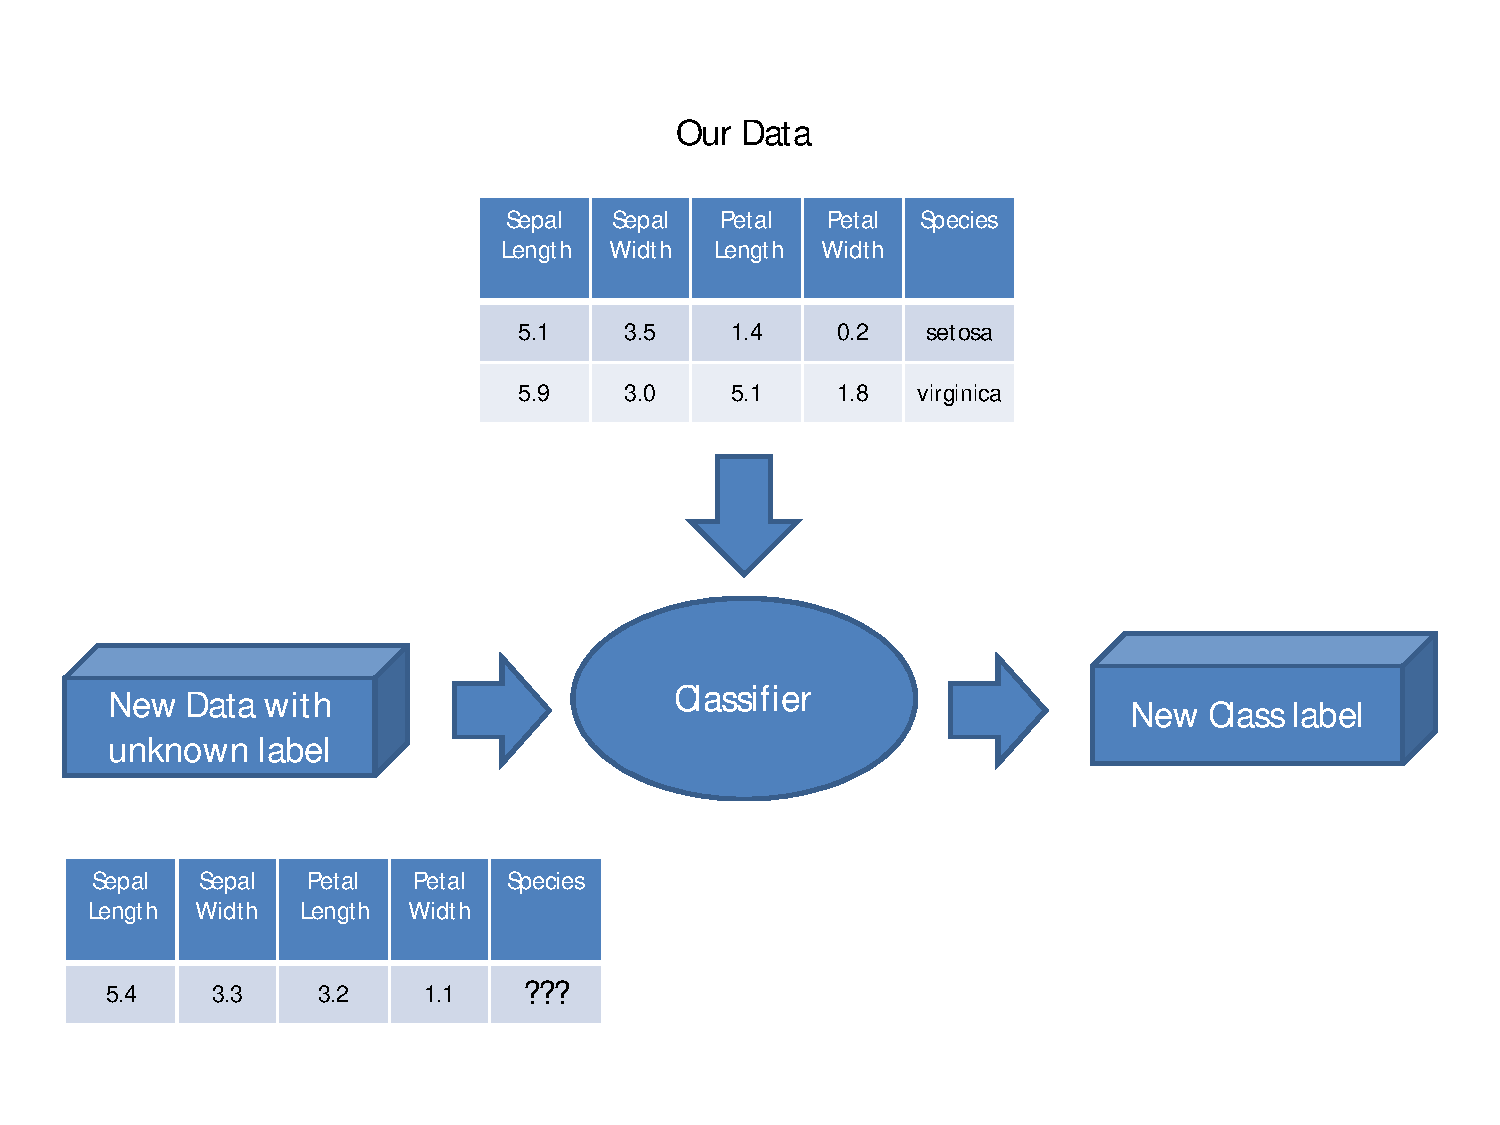
\includegraphics[width= .7\textwidth]{figure_man/classifier.pdf}}

\end{vbframe}

\begin{vbframe}{Binary and Multiclass Tasks}
The task can contain 2 classes (binary) or multiple (multiclass).
\begin{columns}[T]
  \begin{column}{0.5\textwidth}
\begin{knitrout}\scriptsize
\definecolor{shadecolor}{rgb}{0.969, 0.969, 0.969}\color{fgcolor}

{\centering 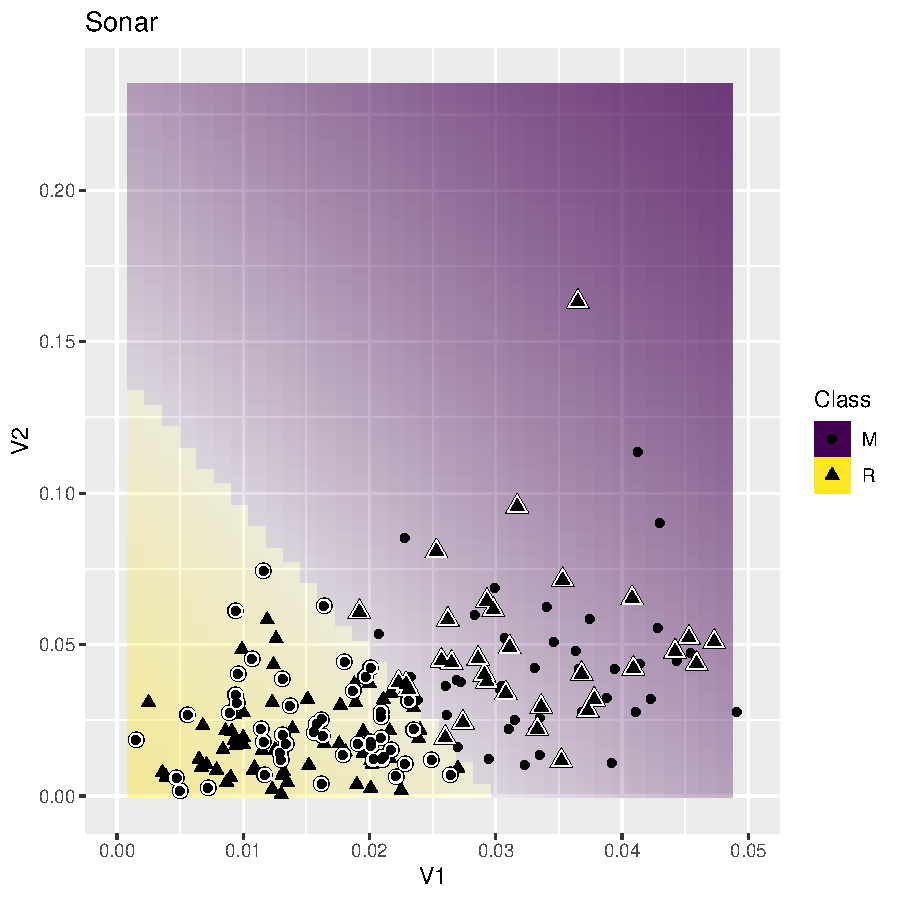
\includegraphics[width=0.95\textwidth]{figure/reg_class_task_1} 

}



\end{knitrout}
  \end{column}
  \begin{column}{0.5\textwidth}
\begin{knitrout}\scriptsize
\definecolor{shadecolor}{rgb}{0.969, 0.969, 0.969}\color{fgcolor}

{\centering 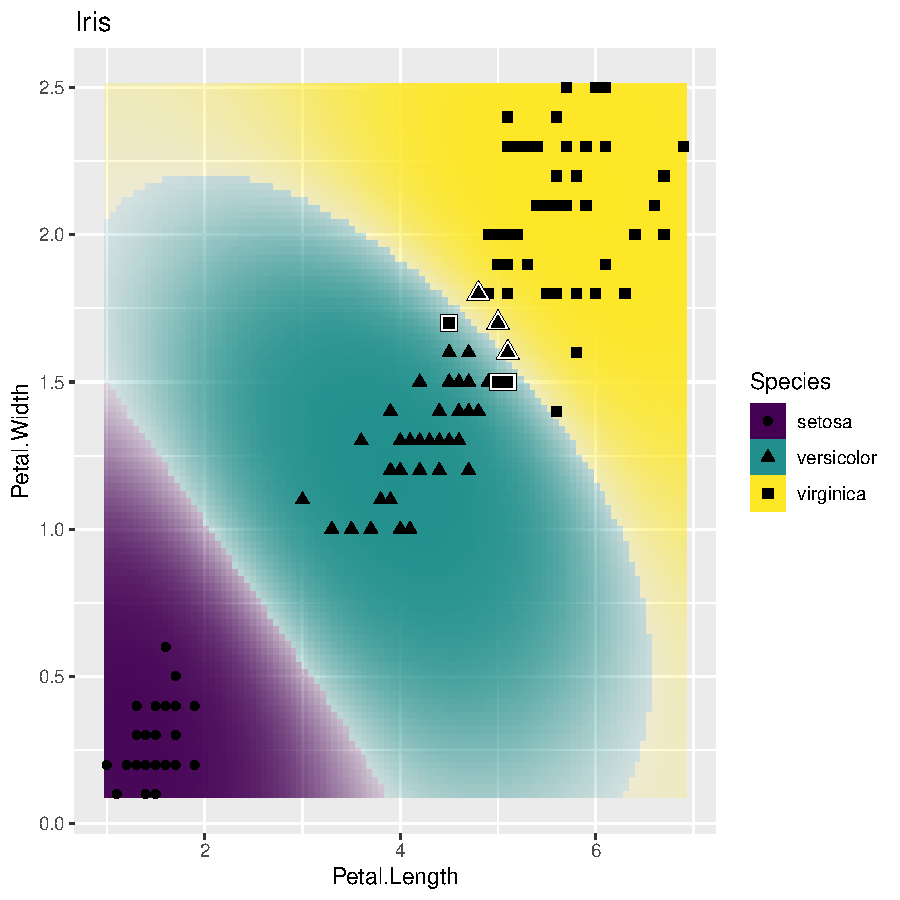
\includegraphics[width=0.95\textwidth]{figure/reg_class_task_2} 

}



\end{knitrout}
  \end{column}
\end{columns}
\end{vbframe}


\begin{vbframe}{Binary Classification Task - Examples}

  \begin{itemize}
  \item Credit risk prediction, based on personal data and transactions 
  \item Spam detection based on textual features 
  \item Churn prediction based on customer behavior
  \item Predisposition for specific illness based on genetic data
  % \item $\ldots$
\end{itemize}

\begin{center}
  % FIGURE SOURCE: https://www.bendbulletin.com/localstate/deschutescounty/3430324-151/fact-or-fiction-polygraphs-just-an-investigative-tool
  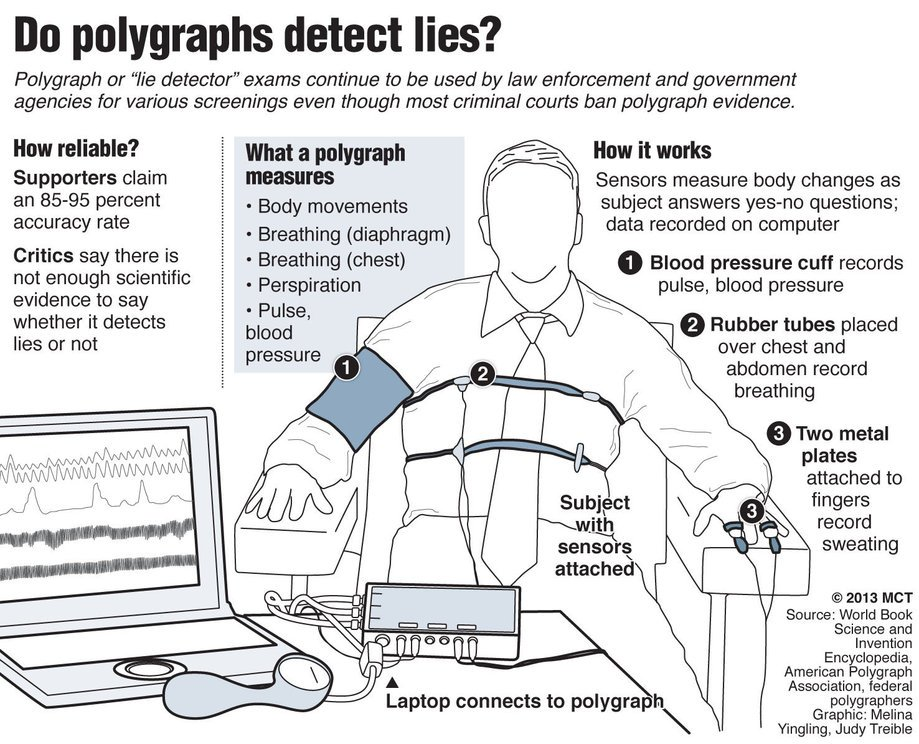
\includegraphics[width=0.6\textwidth]{figure_man/lie-detector-polygraph.jpg}
\end{center}
\vspace{-0.6cm}
\begin{flushright}
  \tiny https://www.bendbulletin.com/localstate/deschutescounty/3430324-151/fact-or-fiction-polygraphs-just-an-investigative-tool
\end{flushright}
\end{vbframe}



\begin{vbframe}{Multiclass Task - Medical Diagnosis}
\begin{center}
  % FIGURE SOURCE: https://symptoms.webmd.com
  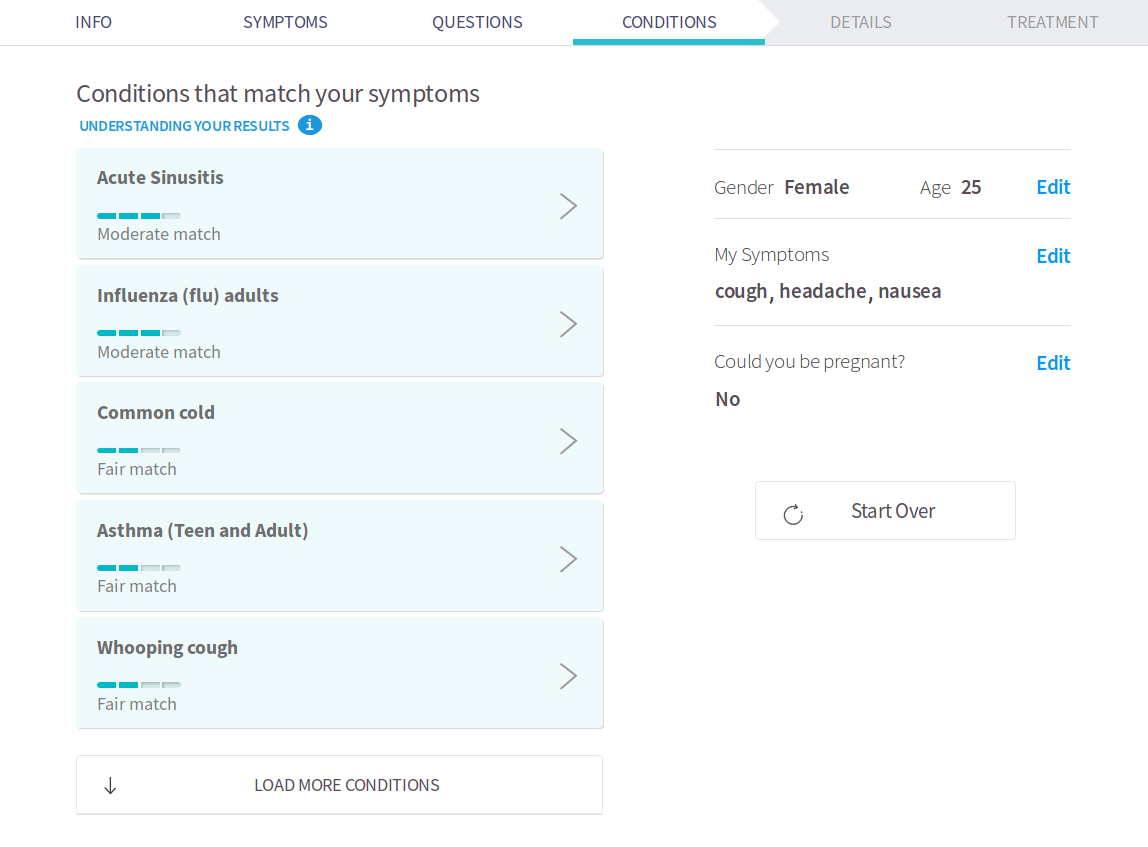
\includegraphics[width=0.8\textwidth]{figure_man/webmd.png}
\end{center}
\vspace{-0.5cm}
\begin{flushright}
  \tiny https://symptoms.webmd.com
\end{flushright}
\end{vbframe}

\begin{vbframe}{Multiclass Task - Iris}

The iris dataset was introduced by the statistician Ronald Fisher and is one
of the most frequent used datasets. Originally it was designed for linear
discriminant analysis.

\begin{center}
\parbox{0.3\textwidth}{
\centering
  \begin{tabular}{@{}c@{}}
    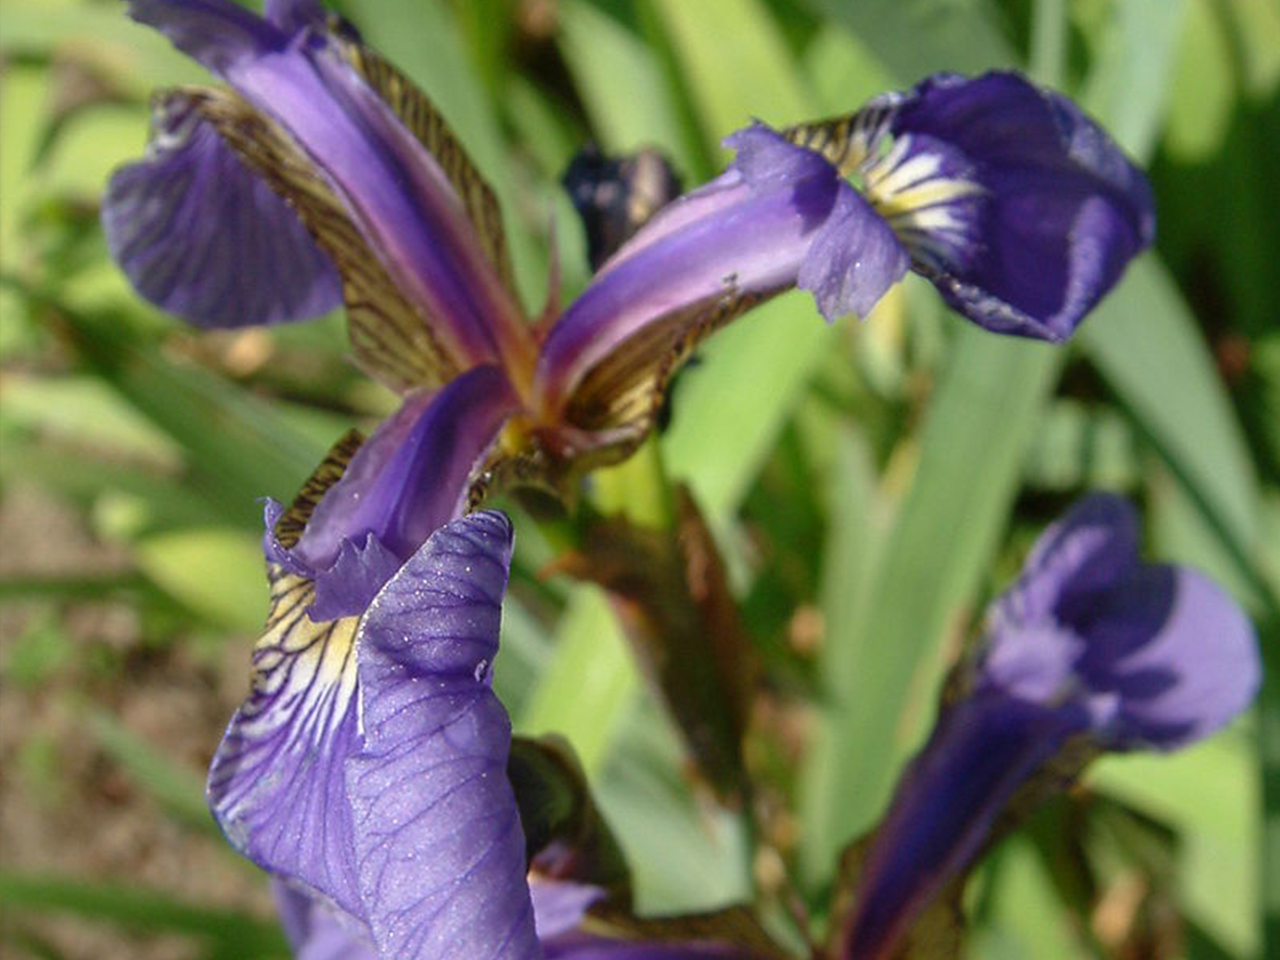
\includegraphics[width=0.25\textwidth]{figure_man/iris_setosa.jpg} \\[\abovecaptionskip]
    \small Setosa
  \end{tabular}
}
\parbox{0.3\textwidth}{
\centering
  \begin{tabular}{@{}c@{}}
    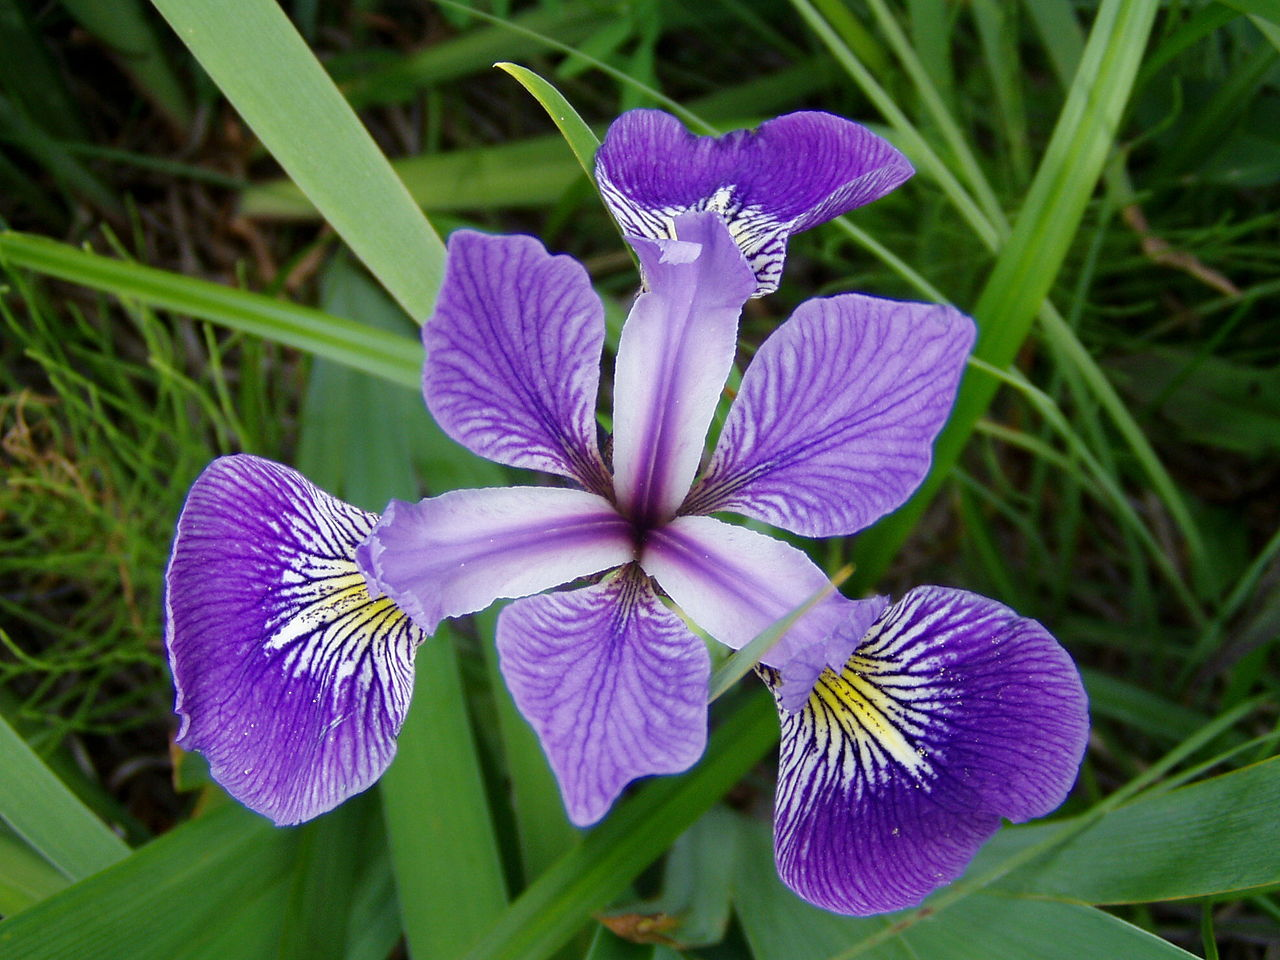
\includegraphics[width=0.25\textwidth]{figure_man/iris_versicolor.jpg} \\[\abovecaptionskip]
    \small Versicolor
  \end{tabular}
}
\parbox{0.3\textwidth}{
\centering
  \begin{tabular}{@{}c@{}}
    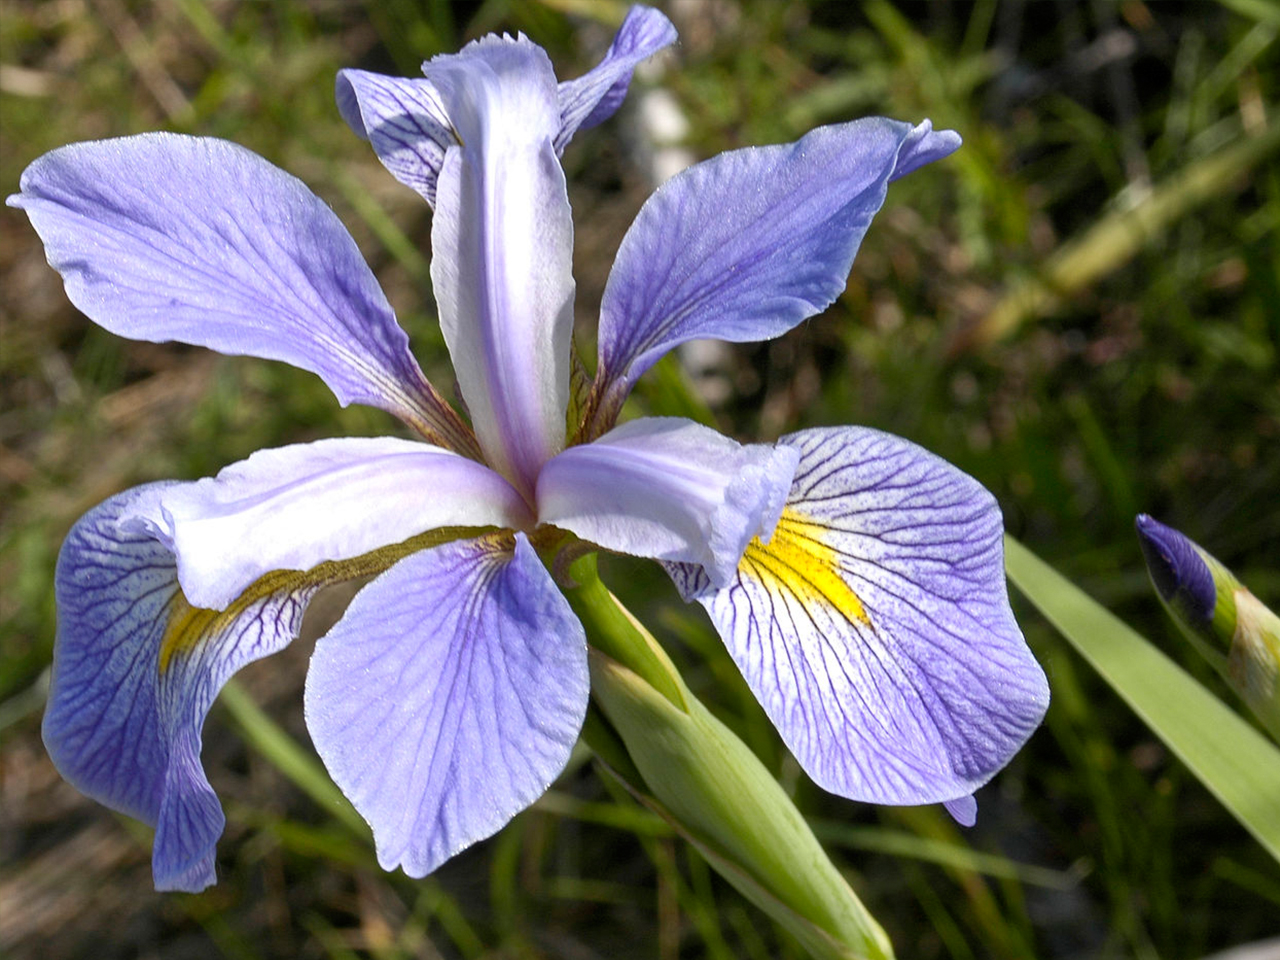
\includegraphics[width=0.25\textwidth]{figure_man/iris_virginica.jpg} \\[\abovecaptionskip]
    \small Virginica
  \end{tabular}
}
\end{center}
  Source: \url{https://en.wikipedia.org/wiki/Iris\_flower\_data\_set}
\end{vbframe}

\begin{vbframe}{Multiclass Task - Iris}

\begin{columns}[T]
\begin{column}{0.5\textwidth}
\begin{itemize}
\item 150 iris flowers 
\item Predict subspecies
\item Based on sepal and petal length / width in [cm]
\end{itemize}
\end{column}
\begin{column}{0.5\textwidth}
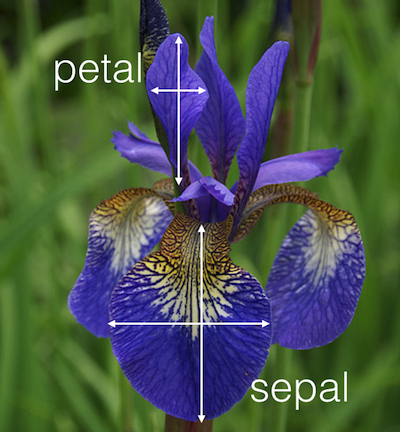
\includegraphics[width=0.4\textwidth]{figure_man/iris_petal_sepal.png} 
\end{column}
\end{columns}
\begin{knitrout}\scriptsize
\definecolor{shadecolor}{rgb}{0.969, 0.969, 0.969}\color{fgcolor}\begin{kframe}
\begin{verbatim}
##      Sepal.Length Sepal.Width Petal.Length Petal.Width   Species
##   1:          5.1         3.5          1.4         0.2    setosa
##   2:          4.9         3.0          1.4         0.2    setosa
##   3:          4.7         3.2          1.3         0.2    setosa
##   4:          4.6         3.1          1.5         0.2    setosa
##   5:          5.0         3.6          1.4         0.2    setosa
##  ---                                                            
## 146:          6.7         3.0          5.2         2.3 virginica
## 147:          6.3         2.5          5.0         1.9 virginica
## 148:          6.5         3.0          5.2         2.0 virginica
## 149:          6.2         3.4          5.4         2.3 virginica
## 150:          5.9         3.0          5.1         1.8 virginica
\end{verbatim}
\end{kframe}
\end{knitrout}
\end{vbframe}

\begin{vbframe}{Multiclass Task - Iris}
\begin{knitrout}\scriptsize
\definecolor{shadecolor}{rgb}{0.969, 0.969, 0.969}\color{fgcolor}

{\centering 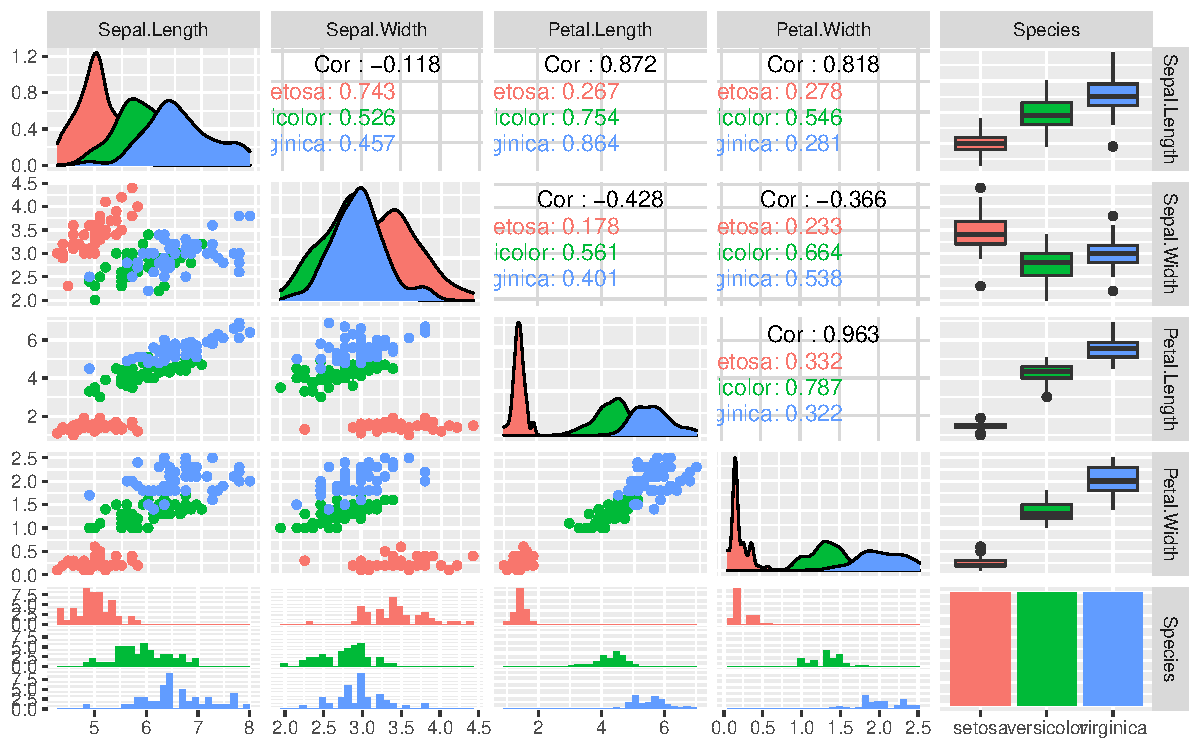
\includegraphics[width=0.95\textwidth]{figure/reg_class_task_3} 

}

\end{knitrout}
\end{vbframe}


\endlecture

\end{document}
